% Created by tikzDevice version 0.7.0 on 2014-01-30 09:59:30
% !TEX encoding = UTF-8 Unicode
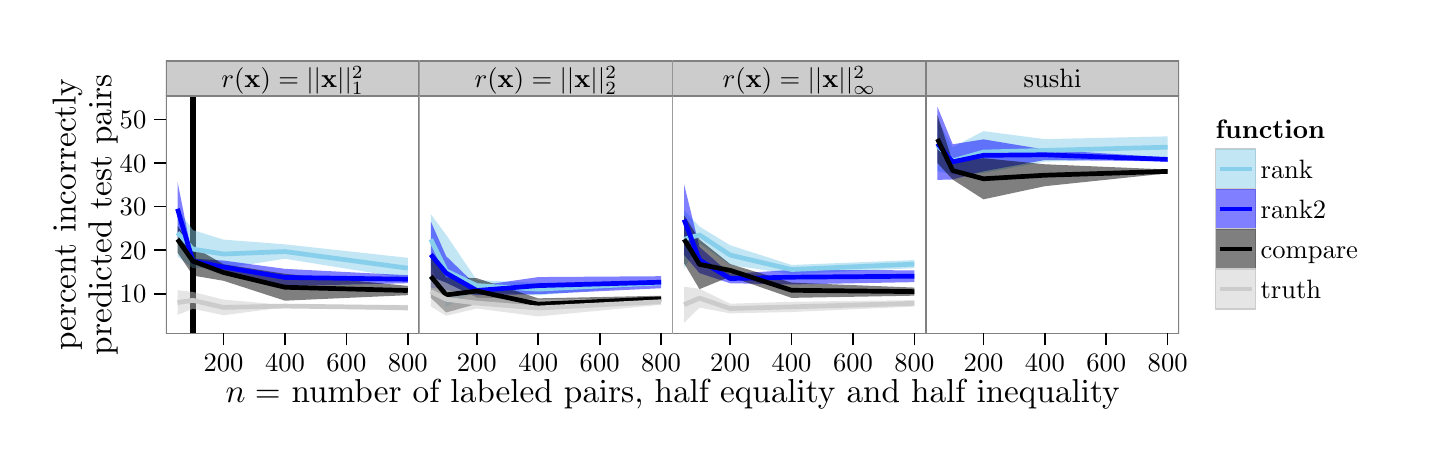
\begin{tikzpicture}[x=1pt,y=1pt]
\definecolor[named]{fillColor}{rgb}{1.00,1.00,1.00}
\path[use as bounding box,fill=fillColor,fill opacity=0.00] (0,0) rectangle (505.89,144.54);
\begin{scope}
\path[clip] (  0.00,  0.00) rectangle (505.89,144.54);
\definecolor[named]{drawColor}{rgb}{1.00,1.00,1.00}
\definecolor[named]{fillColor}{rgb}{1.00,1.00,1.00}

\path[draw=drawColor,line width= 0.6pt,line join=round,line cap=round,fill=fillColor] (  0.00,  0.00) rectangle (505.89,144.54);
\end{scope}
\begin{scope}
\path[clip] ( 49.98,119.86) rectangle (141.51,132.50);
\definecolor[named]{drawColor}{rgb}{0.50,0.50,0.50}
\definecolor[named]{fillColor}{rgb}{0.80,0.80,0.80}

\path[draw=drawColor,line width= 0.6pt,line join=round,line cap=round,fill=fillColor] ( 49.98,119.86) rectangle (141.51,132.50);
\definecolor[named]{drawColor}{rgb}{0.00,0.00,0.00}

\node[text=drawColor,anchor=base,inner sep=0pt, outer sep=0pt, scale=  0.96] at ( 95.74,122.87) {$r(\mathbf x) = ||\mathbf x||_1^2$};
\end{scope}
\begin{scope}
\path[clip] (141.51,119.86) rectangle (233.04,132.50);
\definecolor[named]{drawColor}{rgb}{0.50,0.50,0.50}
\definecolor[named]{fillColor}{rgb}{0.80,0.80,0.80}

\path[draw=drawColor,line width= 0.6pt,line join=round,line cap=round,fill=fillColor] (141.51,119.86) rectangle (233.04,132.50);
\definecolor[named]{drawColor}{rgb}{0.00,0.00,0.00}

\node[text=drawColor,anchor=base,inner sep=0pt, outer sep=0pt, scale=  0.96] at (187.27,122.87) {$r(\mathbf x) = ||\mathbf x||_2^2$};
\end{scope}
\begin{scope}
\path[clip] (233.04,119.86) rectangle (324.57,132.50);
\definecolor[named]{drawColor}{rgb}{0.50,0.50,0.50}
\definecolor[named]{fillColor}{rgb}{0.80,0.80,0.80}

\path[draw=drawColor,line width= 0.6pt,line join=round,line cap=round,fill=fillColor] (233.04,119.86) rectangle (324.57,132.50);
\definecolor[named]{drawColor}{rgb}{0.00,0.00,0.00}

\node[text=drawColor,anchor=base,inner sep=0pt, outer sep=0pt, scale=  0.96] at (278.80,122.87) {$r(\mathbf x) = ||\mathbf x||_\infty^2$};
\end{scope}
\begin{scope}
\path[clip] (324.57,119.86) rectangle (416.09,132.50);
\definecolor[named]{drawColor}{rgb}{0.50,0.50,0.50}
\definecolor[named]{fillColor}{rgb}{0.80,0.80,0.80}

\path[draw=drawColor,line width= 0.6pt,line join=round,line cap=round,fill=fillColor] (324.57,119.86) rectangle (416.09,132.50);
\definecolor[named]{drawColor}{rgb}{0.00,0.00,0.00}

\node[text=drawColor,anchor=base,inner sep=0pt, outer sep=0pt, scale=  0.96] at (370.33,122.87) {sushi};
\end{scope}
\begin{scope}
\path[clip] ( 49.98, 34.03) rectangle (141.51,119.86);
\definecolor[named]{fillColor}{rgb}{1.00,1.00,1.00}

\path[fill=fillColor] ( 49.98, 34.03) rectangle (141.51,119.86);
\definecolor[named]{drawColor}{rgb}{0.00,0.00,0.00}
\definecolor[named]{fillColor}{rgb}{0.00,0.00,0.00}

\path[draw=drawColor,line width= 2.3pt,line join=round,fill=fillColor] ( 59.69, 34.03) -- ( 59.69,119.86);
\definecolor[named]{fillColor}{rgb}{0.53,0.81,0.92}

\path[fill=fillColor,fill opacity=0.50] ( 54.14, 78.97) --
	( 59.69, 71.38) --
	( 70.78, 67.96) --
	( 92.97, 66.24) --
	(137.35, 61.38) --
	(137.35, 53.88) --
	( 92.97, 61.04) --
	( 70.78, 57.55) --
	( 59.69, 57.67) --
	( 54.14, 61.90) --
	cycle;
\definecolor[named]{fillColor}{rgb}{0.00,0.00,1.00}

\path[fill=fillColor,fill opacity=0.50] ( 54.14, 88.86) --
	( 59.69, 61.10) --
	( 70.78, 60.38) --
	( 92.97, 57.39) --
	(137.35, 55.08) --
	(137.35, 52.21) --
	( 92.97, 51.18) --
	( 70.78, 55.67) --
	( 59.69, 59.28) --
	( 54.14, 69.35) --
	cycle;
\definecolor[named]{fillColor}{rgb}{0.00,0.00,0.00}

\path[fill=fillColor,fill opacity=0.50] ( 54.14, 72.80) --
	( 59.69, 65.42) --
	( 70.78, 59.03) --
	( 92.97, 55.58) --
	(137.35, 51.23) --
	(137.35, 47.88) --
	( 92.97, 45.89) --
	( 70.78, 53.08) --
	( 59.69, 54.97) --
	( 54.14, 63.34) --
	cycle;
\definecolor[named]{fillColor}{rgb}{0.80,0.80,0.80}

\path[fill=fillColor,fill opacity=0.50] ( 54.14, 49.68) --
	( 59.69, 49.03) --
	( 70.78, 46.28) --
	( 92.97, 44.32) --
	(137.35, 44.37) --
	(137.35, 42.33) --
	( 92.97, 43.56) --
	( 70.78, 40.62) --
	( 59.69, 42.99) --
	( 54.14, 40.76) --
	cycle;
\definecolor[named]{drawColor}{rgb}{0.53,0.81,0.92}

\path[draw=drawColor,line width= 1.7pt,line join=round] ( 54.14, 70.44) --
	( 59.69, 64.53) --
	( 70.78, 62.75) --
	( 92.97, 63.64) --
	(137.35, 57.63);
\definecolor[named]{drawColor}{rgb}{0.00,0.00,1.00}

\path[draw=drawColor,line width= 1.7pt,line join=round] ( 54.14, 79.10) --
	( 59.69, 60.19) --
	( 70.78, 58.03) --
	( 92.97, 54.28) --
	(137.35, 53.64);
\definecolor[named]{drawColor}{rgb}{0.00,0.00,0.00}

\path[draw=drawColor,line width= 1.7pt,line join=round] ( 54.14, 68.07) --
	( 59.69, 60.19) --
	( 70.78, 56.06) --
	( 92.97, 50.74) --
	(137.35, 49.56);
\definecolor[named]{drawColor}{rgb}{0.80,0.80,0.80}

\path[draw=drawColor,line width= 1.7pt,line join=round] ( 54.14, 45.22) --
	( 59.69, 46.01) --
	( 70.78, 43.45) --
	( 92.97, 43.94) --
	(137.35, 43.35);
\definecolor[named]{drawColor}{rgb}{0.50,0.50,0.50}

\path[draw=drawColor,line width= 0.6pt,line join=round,line cap=round] ( 49.98, 34.03) rectangle (141.51,119.86);
\end{scope}
\begin{scope}
\path[clip] (141.51, 34.03) rectangle (233.04,119.86);
\definecolor[named]{fillColor}{rgb}{1.00,1.00,1.00}

\path[fill=fillColor] (141.51, 34.03) rectangle (233.04,119.86);
\definecolor[named]{fillColor}{rgb}{0.53,0.81,0.92}

\path[fill=fillColor,fill opacity=0.50] (145.67, 77.13) --
	(151.22, 69.67) --
	(162.31, 53.30) --
	(184.50, 52.29) --
	(228.88, 52.87) --
	(228.88, 51.76) --
	(184.50, 47.81) --
	(162.31, 49.36) --
	(151.22, 43.63) --
	(145.67, 59.02) --
	cycle;
\definecolor[named]{fillColor}{rgb}{0.00,0.00,1.00}

\path[fill=fillColor,fill opacity=0.50] (145.67, 74.49) --
	(151.22, 61.95) --
	(162.31, 51.20) --
	(184.50, 54.42) --
	(228.88, 54.73) --
	(228.88, 50.39) --
	(184.50, 48.23) --
	(162.31, 47.91) --
	(151.22, 49.77) --
	(145.67, 50.62) --
	cycle;
\definecolor[named]{fillColor}{rgb}{0.00,0.00,0.00}

\path[fill=fillColor,fill opacity=0.50] (145.67, 62.40) --
	(151.22, 54.33) --
	(162.31, 54.01) --
	(184.50, 46.73) --
	(228.88, 47.67) --
	(228.88, 45.43) --
	(184.50, 42.53) --
	(162.31, 44.70) --
	(151.22, 41.63) --
	(145.67, 46.96) --
	cycle;
\definecolor[named]{fillColor}{rgb}{0.80,0.80,0.80}

\path[fill=fillColor,fill opacity=0.50] (145.67, 54.54) --
	(151.22, 52.35) --
	(162.31, 46.99) --
	(184.50, 46.30) --
	(228.88, 46.65) --
	(228.88, 44.39) --
	(184.50, 40.20) --
	(162.31, 43.05) --
	(151.22, 40.45) --
	(145.67, 43.78) --
	cycle;
\definecolor[named]{drawColor}{rgb}{0.53,0.81,0.92}

\path[draw=drawColor,line width= 1.7pt,line join=round] (145.67, 68.07) --
	(151.22, 56.65) --
	(162.31, 51.33) --
	(184.50, 50.05) --
	(228.88, 52.31);
\definecolor[named]{drawColor}{rgb}{0.00,0.00,1.00}

\path[draw=drawColor,line width= 1.7pt,line join=round] (145.67, 62.56) --
	(151.22, 55.86) --
	(162.31, 49.56) --
	(184.50, 51.33) --
	(228.88, 52.56);
\definecolor[named]{drawColor}{rgb}{0.00,0.00,0.00}

\path[draw=drawColor,line width= 1.7pt,line join=round] (145.67, 54.68) --
	(151.22, 47.98) --
	(162.31, 49.36) --
	(184.50, 44.63) --
	(228.88, 46.55);
\definecolor[named]{drawColor}{rgb}{0.80,0.80,0.80}

\path[draw=drawColor,line width= 1.7pt,line join=round] (145.67, 49.16) --
	(151.22, 46.40) --
	(162.31, 45.02) --
	(184.50, 43.25) --
	(228.88, 45.52);
\definecolor[named]{drawColor}{rgb}{0.50,0.50,0.50}

\path[draw=drawColor,line width= 0.6pt,line join=round,line cap=round] (141.51, 34.03) rectangle (233.04,119.86);
\end{scope}
\begin{scope}
\path[clip] (233.04, 34.03) rectangle (324.57,119.86);
\definecolor[named]{fillColor}{rgb}{1.00,1.00,1.00}

\path[fill=fillColor] (233.04, 34.03) rectangle (324.57,119.86);
\definecolor[named]{fillColor}{rgb}{0.53,0.81,0.92}

\path[fill=fillColor,fill opacity=0.50] (237.20, 78.49) --
	(242.75, 72.67) --
	(253.84, 65.91) --
	(276.03, 58.79) --
	(320.41, 60.57) --
	(320.41, 57.65) --
	(276.03, 55.49) --
	(253.84, 58.81) --
	(242.75, 66.63) --
	(237.20, 57.66) --
	cycle;
\definecolor[named]{fillColor}{rgb}{0.00,0.00,1.00}

\path[fill=fillColor,fill opacity=0.50] (237.20, 87.90) --
	(242.75, 65.29) --
	(253.84, 55.59) --
	(276.03, 57.00) --
	(320.41, 56.86) --
	(320.41, 52.59) --
	(276.03, 51.76) --
	(253.84, 52.19) --
	(242.75, 55.88) --
	(237.20, 62.43) --
	cycle;
\definecolor[named]{fillColor}{rgb}{0.00,0.00,0.00}

\path[fill=fillColor,fill opacity=0.50] (237.20, 76.75) --
	(242.75, 67.96) --
	(253.84, 59.11) --
	(276.03, 52.41) --
	(320.41, 50.62) --
	(320.41, 47.70) --
	(276.03, 46.90) --
	(253.84, 54.58) --
	(242.75, 50.06) --
	(237.20, 59.39) --
	cycle;
\definecolor[named]{fillColor}{rgb}{0.80,0.80,0.80}

\path[fill=fillColor,fill opacity=0.50] (237.20, 50.93) --
	(242.75, 50.20) --
	(253.84, 44.80) --
	(276.03, 45.49) --
	(320.41, 46.09) --
	(320.41, 43.76) --
	(276.03, 41.80) --
	(253.84, 41.31) --
	(242.75, 43.39) --
	(237.20, 37.94) --
	cycle;
\definecolor[named]{drawColor}{rgb}{0.53,0.81,0.92}

\path[draw=drawColor,line width= 1.7pt,line join=round] (237.20, 68.07) --
	(242.75, 69.65) --
	(253.84, 62.36) --
	(276.03, 57.14) --
	(320.41, 59.11);
\definecolor[named]{drawColor}{rgb}{0.00,0.00,1.00}

\path[draw=drawColor,line width= 1.7pt,line join=round] (237.20, 75.16) --
	(242.75, 60.59) --
	(253.84, 53.89) --
	(276.03, 54.38) --
	(320.41, 54.73);
\definecolor[named]{drawColor}{rgb}{0.00,0.00,0.00}

\path[draw=drawColor,line width= 1.7pt,line join=round] (237.20, 68.07) --
	(242.75, 59.01) --
	(253.84, 56.84) --
	(276.03, 49.65) --
	(320.41, 49.16);
\definecolor[named]{drawColor}{rgb}{0.80,0.80,0.80}

\path[draw=drawColor,line width= 1.7pt,line join=round] (237.20, 44.43) --
	(242.75, 46.80) --
	(253.84, 43.05) --
	(276.03, 43.65) --
	(320.41, 44.93);
\definecolor[named]{drawColor}{rgb}{0.50,0.50,0.50}

\path[draw=drawColor,line width= 0.6pt,line join=round,line cap=round] (233.04, 34.03) rectangle (324.57,119.86);
\end{scope}
\begin{scope}
\path[clip] (324.57, 34.03) rectangle (416.09,119.86);
\definecolor[named]{fillColor}{rgb}{1.00,1.00,1.00}

\path[fill=fillColor] (324.57, 34.03) rectangle (416.09,119.86);
\definecolor[named]{fillColor}{rgb}{0.53,0.81,0.92}

\path[fill=fillColor,fill opacity=0.50] (328.73,111.23) --
	(334.27,101.34) --
	(345.37,107.15) --
	(367.56,104.26) --
	(411.93,105.26) --
	(411.93, 97.46) --
	(367.56, 96.11) --
	(345.37, 92.03) --
	(334.27, 91.54) --
	(328.73, 92.68) --
	cycle;
\definecolor[named]{fillColor}{rgb}{0.00,0.00,1.00}

\path[fill=fillColor,fill opacity=0.50] (328.73,115.96) --
	(334.27,102.40) --
	(345.37,104.18) --
	(367.56,100.50) --
	(411.93, 97.63) --
	(411.93, 96.24) --
	(367.56, 96.72) --
	(345.37, 92.64) --
	(334.27, 89.69) --
	(328.73, 89.53) --
	cycle;
\definecolor[named]{fillColor}{rgb}{0.00,0.00,0.00}

\path[fill=fillColor,fill opacity=0.50] (328.73,113.00) --
	(334.27, 96.14) --
	(345.37, 97.37) --
	(367.56, 95.18) --
	(411.93, 93.29) --
	(411.93, 91.90) --
	(367.56, 87.26) --
	(345.37, 82.51) --
	(334.27, 89.64) --
	(328.73, 95.64) --
	cycle;
\definecolor[named]{drawColor}{rgb}{0.53,0.81,0.92}

\path[draw=drawColor,line width= 1.7pt,line join=round] (328.73,101.96) --
	(334.27, 96.44) --
	(345.37, 99.59) --
	(367.56,100.18) --
	(411.93,101.36);
\definecolor[named]{drawColor}{rgb}{0.00,0.00,1.00}

\path[draw=drawColor,line width= 1.7pt,line join=round] (328.73,102.74) --
	(334.27, 96.05) --
	(345.37, 98.41) --
	(367.56, 98.61) --
	(411.93, 96.93);
\definecolor[named]{drawColor}{rgb}{0.00,0.00,0.00}

\path[draw=drawColor,line width= 1.7pt,line join=round] (328.73,104.32) --
	(334.27, 92.89) --
	(345.37, 89.94) --
	(367.56, 91.22) --
	(411.93, 92.60);
\definecolor[named]{drawColor}{rgb}{0.50,0.50,0.50}

\path[draw=drawColor,line width= 0.6pt,line join=round,line cap=round] (324.57, 34.03) rectangle (416.09,119.86);
\end{scope}
\begin{scope}
\path[clip] (  0.00,  0.00) rectangle (505.89,144.54);
\definecolor[named]{drawColor}{rgb}{0.00,0.00,0.00}

\node[text=drawColor,anchor=base east,inner sep=0pt, outer sep=0pt, scale=  0.96] at ( 42.87, 45.07) {10};

\node[text=drawColor,anchor=base east,inner sep=0pt, outer sep=0pt, scale=  0.96] at ( 42.87, 60.83) {20};

\node[text=drawColor,anchor=base east,inner sep=0pt, outer sep=0pt, scale=  0.96] at ( 42.87, 76.59) {30};

\node[text=drawColor,anchor=base east,inner sep=0pt, outer sep=0pt, scale=  0.96] at ( 42.87, 92.35) {40};

\node[text=drawColor,anchor=base east,inner sep=0pt, outer sep=0pt, scale=  0.96] at ( 42.87,108.10) {50};
\end{scope}
\begin{scope}
\path[clip] (  0.00,  0.00) rectangle (505.89,144.54);
\definecolor[named]{drawColor}{rgb}{0.00,0.00,0.00}

\path[draw=drawColor,line width= 0.6pt,line join=round] ( 45.71, 48.37) --
	( 49.98, 48.37);

\path[draw=drawColor,line width= 0.6pt,line join=round] ( 45.71, 64.13) --
	( 49.98, 64.13);

\path[draw=drawColor,line width= 0.6pt,line join=round] ( 45.71, 79.89) --
	( 49.98, 79.89);

\path[draw=drawColor,line width= 0.6pt,line join=round] ( 45.71, 95.65) --
	( 49.98, 95.65);

\path[draw=drawColor,line width= 0.6pt,line join=round] ( 45.71,111.41) --
	( 49.98,111.41);
\end{scope}
\begin{scope}
\path[clip] (  0.00,  0.00) rectangle (505.89,144.54);
\definecolor[named]{drawColor}{rgb}{0.00,0.00,0.00}

\path[draw=drawColor,line width= 0.6pt,line join=round] ( 70.78, 29.77) --
	( 70.78, 34.03);

\path[draw=drawColor,line width= 0.6pt,line join=round] ( 92.97, 29.77) --
	( 92.97, 34.03);

\path[draw=drawColor,line width= 0.6pt,line join=round] (115.16, 29.77) --
	(115.16, 34.03);

\path[draw=drawColor,line width= 0.6pt,line join=round] (137.35, 29.77) --
	(137.35, 34.03);
\end{scope}
\begin{scope}
\path[clip] (  0.00,  0.00) rectangle (505.89,144.54);
\definecolor[named]{drawColor}{rgb}{0.00,0.00,0.00}

\node[text=drawColor,anchor=base,inner sep=0pt, outer sep=0pt, scale=  0.96] at ( 70.78, 20.31) {200};

\node[text=drawColor,anchor=base,inner sep=0pt, outer sep=0pt, scale=  0.96] at ( 92.97, 20.31) {400};

\node[text=drawColor,anchor=base,inner sep=0pt, outer sep=0pt, scale=  0.96] at (115.16, 20.31) {600};

\node[text=drawColor,anchor=base,inner sep=0pt, outer sep=0pt, scale=  0.96] at (137.35, 20.31) {800};
\end{scope}
\begin{scope}
\path[clip] (  0.00,  0.00) rectangle (505.89,144.54);
\definecolor[named]{drawColor}{rgb}{0.00,0.00,0.00}

\path[draw=drawColor,line width= 0.6pt,line join=round] (162.31, 29.77) --
	(162.31, 34.03);

\path[draw=drawColor,line width= 0.6pt,line join=round] (184.50, 29.77) --
	(184.50, 34.03);

\path[draw=drawColor,line width= 0.6pt,line join=round] (206.69, 29.77) --
	(206.69, 34.03);

\path[draw=drawColor,line width= 0.6pt,line join=round] (228.88, 29.77) --
	(228.88, 34.03);
\end{scope}
\begin{scope}
\path[clip] (  0.00,  0.00) rectangle (505.89,144.54);
\definecolor[named]{drawColor}{rgb}{0.00,0.00,0.00}

\node[text=drawColor,anchor=base,inner sep=0pt, outer sep=0pt, scale=  0.96] at (162.31, 20.31) {200};

\node[text=drawColor,anchor=base,inner sep=0pt, outer sep=0pt, scale=  0.96] at (184.50, 20.31) {400};

\node[text=drawColor,anchor=base,inner sep=0pt, outer sep=0pt, scale=  0.96] at (206.69, 20.31) {600};

\node[text=drawColor,anchor=base,inner sep=0pt, outer sep=0pt, scale=  0.96] at (228.88, 20.31) {800};
\end{scope}
\begin{scope}
\path[clip] (  0.00,  0.00) rectangle (505.89,144.54);
\definecolor[named]{drawColor}{rgb}{0.00,0.00,0.00}

\path[draw=drawColor,line width= 0.6pt,line join=round] (253.84, 29.77) --
	(253.84, 34.03);

\path[draw=drawColor,line width= 0.6pt,line join=round] (276.03, 29.77) --
	(276.03, 34.03);

\path[draw=drawColor,line width= 0.6pt,line join=round] (298.22, 29.77) --
	(298.22, 34.03);

\path[draw=drawColor,line width= 0.6pt,line join=round] (320.41, 29.77) --
	(320.41, 34.03);
\end{scope}
\begin{scope}
\path[clip] (  0.00,  0.00) rectangle (505.89,144.54);
\definecolor[named]{drawColor}{rgb}{0.00,0.00,0.00}

\node[text=drawColor,anchor=base,inner sep=0pt, outer sep=0pt, scale=  0.96] at (253.84, 20.31) {200};

\node[text=drawColor,anchor=base,inner sep=0pt, outer sep=0pt, scale=  0.96] at (276.03, 20.31) {400};

\node[text=drawColor,anchor=base,inner sep=0pt, outer sep=0pt, scale=  0.96] at (298.22, 20.31) {600};

\node[text=drawColor,anchor=base,inner sep=0pt, outer sep=0pt, scale=  0.96] at (320.41, 20.31) {800};
\end{scope}
\begin{scope}
\path[clip] (  0.00,  0.00) rectangle (505.89,144.54);
\definecolor[named]{drawColor}{rgb}{0.00,0.00,0.00}

\path[draw=drawColor,line width= 0.6pt,line join=round] (345.37, 29.77) --
	(345.37, 34.03);

\path[draw=drawColor,line width= 0.6pt,line join=round] (367.56, 29.77) --
	(367.56, 34.03);

\path[draw=drawColor,line width= 0.6pt,line join=round] (389.75, 29.77) --
	(389.75, 34.03);

\path[draw=drawColor,line width= 0.6pt,line join=round] (411.93, 29.77) --
	(411.93, 34.03);
\end{scope}
\begin{scope}
\path[clip] (  0.00,  0.00) rectangle (505.89,144.54);
\definecolor[named]{drawColor}{rgb}{0.00,0.00,0.00}

\node[text=drawColor,anchor=base,inner sep=0pt, outer sep=0pt, scale=  0.96] at (345.37, 20.31) {200};

\node[text=drawColor,anchor=base,inner sep=0pt, outer sep=0pt, scale=  0.96] at (367.56, 20.31) {400};

\node[text=drawColor,anchor=base,inner sep=0pt, outer sep=0pt, scale=  0.96] at (389.75, 20.31) {600};

\node[text=drawColor,anchor=base,inner sep=0pt, outer sep=0pt, scale=  0.96] at (411.93, 20.31) {800};
\end{scope}
\begin{scope}
\path[clip] (  0.00,  0.00) rectangle (505.89,144.54);
\definecolor[named]{drawColor}{rgb}{0.00,0.00,0.00}

\node[text=drawColor,anchor=base,inner sep=0pt, outer sep=0pt, scale=  1.20] at (233.04,  9.03) {$n=$ number of labeled pairs, half equality and half inequality};
\end{scope}
\begin{scope}
\path[clip] (  0.00,  0.00) rectangle (505.89,144.54);
\definecolor[named]{drawColor}{rgb}{0.00,0.00,0.00}

\node[text=drawColor,rotate= 90.00,anchor=base,inner sep=0pt, outer sep=0pt, scale=  1.20] at ( 17.30, 76.95) {percent incorrectly};

\node[text=drawColor,rotate= 90.00,anchor=base,inner sep=0pt, outer sep=0pt, scale=  1.20] at ( 30.26, 76.95) {predicted test pairs};
\end{scope}
\begin{scope}
\path[clip] (  0.00,  0.00) rectangle (505.89,144.54);
\definecolor[named]{fillColor}{rgb}{1.00,1.00,1.00}

\path[fill=fillColor] (424.96, 38.65) rectangle (484.98,115.24);
\end{scope}
\begin{scope}
\path[clip] (  0.00,  0.00) rectangle (505.89,144.54);
\definecolor[named]{drawColor}{rgb}{0.00,0.00,0.00}

\node[text=drawColor,anchor=base west,inner sep=0pt, outer sep=0pt, scale=  0.96] at (429.23,104.35) {\bfseries function};
\end{scope}
\begin{scope}
\path[clip] (  0.00,  0.00) rectangle (505.89,144.54);
\definecolor[named]{drawColor}{rgb}{0.80,0.80,0.80}
\definecolor[named]{fillColor}{rgb}{1.00,1.00,1.00}

\path[draw=drawColor,line width= 0.6pt,line join=round,line cap=round,fill=fillColor] (429.23, 86.28) rectangle (443.68,100.74);
\end{scope}
\begin{scope}
\path[clip] (  0.00,  0.00) rectangle (505.89,144.54);
\definecolor[named]{fillColor}{rgb}{0.53,0.81,0.92}

\path[fill=fillColor,fill opacity=0.50] (429.23, 86.28) rectangle (443.68,100.74);

\path[] (429.23, 86.28) --
	(443.68,100.74);
\end{scope}
\begin{scope}
\path[clip] (  0.00,  0.00) rectangle (505.89,144.54);
\definecolor[named]{drawColor}{rgb}{0.53,0.81,0.92}

\path[draw=drawColor,line width= 1.7pt,line join=round] (430.68, 93.51) -- (442.24, 93.51);
\end{scope}
\begin{scope}
\path[clip] (  0.00,  0.00) rectangle (505.89,144.54);
\definecolor[named]{drawColor}{rgb}{0.80,0.80,0.80}
\definecolor[named]{fillColor}{rgb}{1.00,1.00,1.00}

\path[draw=drawColor,line width= 0.6pt,line join=round,line cap=round,fill=fillColor] (429.23, 71.83) rectangle (443.68, 86.28);
\end{scope}
\begin{scope}
\path[clip] (  0.00,  0.00) rectangle (505.89,144.54);
\definecolor[named]{fillColor}{rgb}{0.00,0.00,1.00}

\path[fill=fillColor,fill opacity=0.50] (429.23, 71.83) rectangle (443.68, 86.28);

\path[] (429.23, 71.83) --
	(443.68, 86.28);
\end{scope}
\begin{scope}
\path[clip] (  0.00,  0.00) rectangle (505.89,144.54);
\definecolor[named]{drawColor}{rgb}{0.00,0.00,1.00}

\path[draw=drawColor,line width= 1.7pt,line join=round] (430.68, 79.06) -- (442.24, 79.06);
\end{scope}
\begin{scope}
\path[clip] (  0.00,  0.00) rectangle (505.89,144.54);
\definecolor[named]{drawColor}{rgb}{0.80,0.80,0.80}
\definecolor[named]{fillColor}{rgb}{1.00,1.00,1.00}

\path[draw=drawColor,line width= 0.6pt,line join=round,line cap=round,fill=fillColor] (429.23, 57.37) rectangle (443.68, 71.83);
\end{scope}
\begin{scope}
\path[clip] (  0.00,  0.00) rectangle (505.89,144.54);
\definecolor[named]{fillColor}{rgb}{0.00,0.00,0.00}

\path[fill=fillColor,fill opacity=0.50] (429.23, 57.37) rectangle (443.68, 71.83);

\path[] (429.23, 57.37) --
	(443.68, 71.83);
\end{scope}
\begin{scope}
\path[clip] (  0.00,  0.00) rectangle (505.89,144.54);
\definecolor[named]{drawColor}{rgb}{0.00,0.00,0.00}

\path[draw=drawColor,line width= 1.7pt,line join=round] (430.68, 64.60) -- (442.24, 64.60);
\end{scope}
\begin{scope}
\path[clip] (  0.00,  0.00) rectangle (505.89,144.54);
\definecolor[named]{drawColor}{rgb}{0.80,0.80,0.80}
\definecolor[named]{fillColor}{rgb}{1.00,1.00,1.00}

\path[draw=drawColor,line width= 0.6pt,line join=round,line cap=round,fill=fillColor] (429.23, 42.92) rectangle (443.68, 57.37);
\end{scope}
\begin{scope}
\path[clip] (  0.00,  0.00) rectangle (505.89,144.54);
\definecolor[named]{fillColor}{rgb}{0.80,0.80,0.80}

\path[fill=fillColor,fill opacity=0.50] (429.23, 42.92) rectangle (443.68, 57.37);

\path[] (429.23, 42.92) --
	(443.68, 57.37);
\end{scope}
\begin{scope}
\path[clip] (  0.00,  0.00) rectangle (505.89,144.54);
\definecolor[named]{drawColor}{rgb}{0.80,0.80,0.80}

\path[draw=drawColor,line width= 1.7pt,line join=round] (430.68, 50.15) -- (442.24, 50.15);
\end{scope}
\begin{scope}
\path[clip] (  0.00,  0.00) rectangle (505.89,144.54);
\definecolor[named]{drawColor}{rgb}{0.00,0.00,0.00}

\node[text=drawColor,anchor=base west,inner sep=0pt, outer sep=0pt, scale=  0.96] at (445.49, 90.20) {rank};
\end{scope}
\begin{scope}
\path[clip] (  0.00,  0.00) rectangle (505.89,144.54);
\definecolor[named]{drawColor}{rgb}{0.00,0.00,0.00}

\node[text=drawColor,anchor=base west,inner sep=0pt, outer sep=0pt, scale=  0.96] at (445.49, 75.75) {rank2};
\end{scope}
\begin{scope}
\path[clip] (  0.00,  0.00) rectangle (505.89,144.54);
\definecolor[named]{drawColor}{rgb}{0.00,0.00,0.00}

\node[text=drawColor,anchor=base west,inner sep=0pt, outer sep=0pt, scale=  0.96] at (445.49, 61.30) {compare};
\end{scope}
\begin{scope}
\path[clip] (  0.00,  0.00) rectangle (505.89,144.54);
\definecolor[named]{drawColor}{rgb}{0.00,0.00,0.00}

\node[text=drawColor,anchor=base west,inner sep=0pt, outer sep=0pt, scale=  0.96] at (445.49, 46.84) {truth};
\end{scope}
\end{tikzpicture}
